\documentclass{standalone}
\usepackage{tikz}
\begin{document}
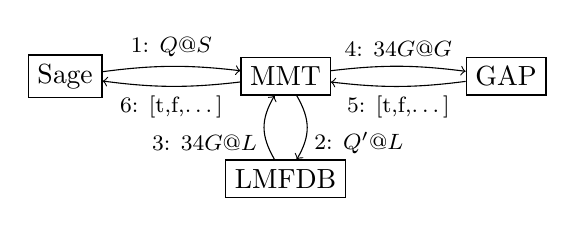
\begin{tikzpicture}[xscale=2.8,yscale=1.3]\normalsize
  \node[draw] (s) at (0,0) {Sage};
  \node[draw] (m) at (1,0) {MMT};
  \node[draw] (g) at (2,0) {GAP};
  \node[draw] (l) at (1,-1) {LMFDB};
  \draw[->] (s) to[bend left=15] node[above] {\footnotesize 1: $Q@S$} (m);
  \draw[->] (m) to[bend left=15] node[right,near end] {\footnotesize 2: $Q'@L$} (l);
  \draw[<-] (m) to[bend right=15] node[left,near end] {\footnotesize 3: $34G@L$} (l);
  \draw[->] (m) to[bend left=15] node[above] {\footnotesize 4: $34G@G$} (g);
  \draw[<-] (m) to[bend right=15] node[below] {\footnotesize 5: [t,f,\ldots]} (g);
  \draw[<-] (s) to[bend right=15] node[below] {\footnotesize 6: [t,f,\ldots]} (m);
\end{tikzpicture}
\end{document}

